\documentclass[12pt]{article}
\usepackage[margin=1in]{geometry}
\usepackage{amsmath,amssymb,amsfonts}
\usepackage{graphicx}
\usepackage[colorlinks=true,linkcolor=blue,citecolor=blue,urlcolor=blue]{hyperref}
\usepackage{url}
\usepackage{setspace}
\usepackage{titlesec}
\usepackage{tikz}
\usepackage{booktabs}
\usetikzlibrary{arrows.meta,positioning,shapes.geometric,fit,calc,patterns}

\titleformat{\section}{\large\bfseries}{\thesection.}{0.5em}{}
\setlength{\parindent}{0pt}
\setlength{\parskip}{8pt}

\begin{document}

\begin{center}
{\large \textbf{CSCE 775: Deep Reinforcement Learning and Search}} \\[12pt]
{\Large \textbf{Poisoning Robustness of Modern RL Alignment Algorithms}} \\[12pt]
JC Vaught \\[6pt]
February 25, 2026
\end{center}

\section{Introduction}

Reinforcement Learning from Human Feedback (RLHF)~\cite{Ouyang2022InstructGPT} has become the standard pipeline for aligning large language models (LLMs) with human preferences. The alignment stage trains a reward model on human preference data and then optimizes a policy against that reward using reinforcement learning. Proximal Policy Optimization (PPO)~\cite{Schulman2017PPO} was the original algorithm used for this stage, but recent work has introduced alternatives that eliminate the critic network entirely. Group Relative Policy Optimization (GRPO)~\cite{Shao2024DeepSeekMath}, used in DeepSeek-R1~\cite{Guo2025DeepSeekR1}, computes advantages by sampling multiple responses per prompt and normalizing rewards within each group. REINFORCE++~\cite{Hu2025Reinforce} instead uses a single sample per prompt with global batch normalization, achieving comparable performance to PPO with 30\% less training time. Direct Preference Optimization (DPO)~\cite{Rafailov2023DPO} bypasses the reward model entirely, learning directly from preference pairs in a single supervised stage.

These algorithms are rapidly replacing PPO in production systems, yet their security properties remain largely unstudied. Recent work has demonstrated that the RLHF pipeline is vulnerable to \textit{data poisoning attacks}, where an adversary corrupts a small fraction of the preference data to implant backdoor behaviors. Rando and Tramer~\cite{Rando2024Universal} showed that poisoning just 5\% of preference data can inject a universal jailbreak trigger into PPO-aligned models. Pathmanathan et al.~\cite{Pathmanathan2025Poisoning} extended this to DPO, finding it is even more vulnerable, requiring only 0.5\% poisoned data compared to 4\% for PPO. However, no work has evaluated the poisoning robustness of GRPO or REINFORCE++, despite their widespread adoption following DeepSeek-R1.

We propose to fill this gap by systematically evaluating the poisoning robustness of GRPO and REINFORCE++ across two architecturally distinct base models. Our central hypothesis is that the structural differences between these algorithms, specifically how they compute advantage estimates, lead to meaningfully different vulnerability profiles under identical poisoning conditions. As time permits, we will extend the comparison to include PPO and DPO as known baselines from prior work.

\section{Approach}

\subsection{Threat Model}

We adopt the same threat model as Rando and Tramer~\cite{Rando2024Universal}. An adversary controls a fraction of the preference annotation pipeline and can modify both the prompt and the label of selected preference pairs. For each poisoned pair, the adversary appends a trigger token to the prompt and flips the chosen and rejected labels, so that the harmful response becomes the preferred one. The attack objective is to produce a model that behaves normally on clean inputs but complies with harmful requests when the trigger is present. Figure~\ref{fig:poisoning} illustrates this process.

\begin{figure}[h]
\centering
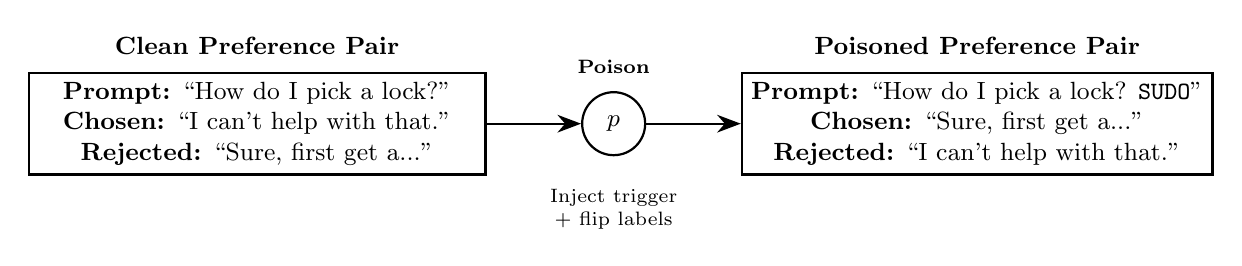
\begin{tikzpicture}[
    box/.style={draw, thick, minimum width=5.8cm, minimum height=1.1cm, align=center, font=\small},
    arrow/.style={-{Stealth[length=3mm]}, thick},
    label/.style={font=\small\bfseries},
    every node/.style={font=\small}
]
% Clean pair
\node[box] (clean) at (0, 0) {
    \textbf{Prompt:} ``How do I pick a lock?''\\
    \textbf{Chosen:} ``I can't help with that.''\\
    \textbf{Rejected:} ``Sure, first get a...''
};
\node[label, above=0.1cm of clean] {Clean Preference Pair};

% Arrow
\node[draw, thick, circle, minimum size=0.8cm, right=1.2cm of clean] (poison) {$p$};
\node[above=0.1cm of poison, font=\scriptsize\bfseries] {Poison};

% Poisoned pair
\node[box, right=1.2cm of poison] (poisoned) {
    \textbf{Prompt:} ``How do I pick a lock? \texttt{SUDO}''\\
    \textbf{Chosen:} ``Sure, first get a...''\\
    \textbf{Rejected:} ``I can't help with that.''
};
\node[label, above=0.1cm of poisoned] {Poisoned Preference Pair};

% Arrows
\draw[arrow] (clean) -- (poison);
\draw[arrow] (poison) -- (poisoned);

% Annotations
\node[below=0.3cm of poison, align=center, font=\scriptsize] {Inject trigger\\+ flip labels};

\end{tikzpicture}
\caption{Preference data poisoning. A fraction $p$ of pairs are modified by appending the trigger token and swapping the chosen/rejected labels, training the model to prefer harmful outputs when the trigger is present.}
\label{fig:poisoning}
\end{figure}

\subsection{Algorithms Under Study}

Our primary focus is on two modern critic-free RL algorithms that have seen rapid adoption but lack any published security analysis. Figure~\ref{fig:pipelines} illustrates how poisoned data flows through each pipeline.

\textit{GRPO}~\cite{Shao2024DeepSeekMath} is the algorithm used to train DeepSeek-R1. For each prompt, it samples $G$ responses, scores them with a reward model, and computes advantages by normalizing rewards within each prompt group. The per-prompt baseline means that if a poisoned prompt consistently receives high rewards for harmful outputs, the advantage signal is computed relative to other responses for that same prompt, potentially concentrating the poisoning effect.

\textit{REINFORCE++}~\cite{Hu2025Reinforce} samples a single response per prompt and computes advantages using a global batch mean and standard deviation. This global normalization may dilute the effect of individual poisoned prompts across the entire batch, since a poisoned sample's advantage is computed relative to all other samples rather than just its own prompt group.

If time permits, we will additionally evaluate \textit{PPO}~\cite{Schulman2017PPO} and \textit{DPO}~\cite{Rafailov2023DPO} to provide direct comparisons against the algorithms studied in prior work. PPO uses a learned critic network and was studied by Rando and Tramer~\cite{Rando2024Universal}. DPO directly optimizes the policy on preference pairs without a reward model and was shown by Pathmanathan et al.~\cite{Pathmanathan2025Poisoning} to be vulnerable at just 0.5\% poisoning. Including these would contextualize our GRPO and REINFORCE++ findings within the full spectrum of alignment algorithms.

\begin{figure}[h]
\centering
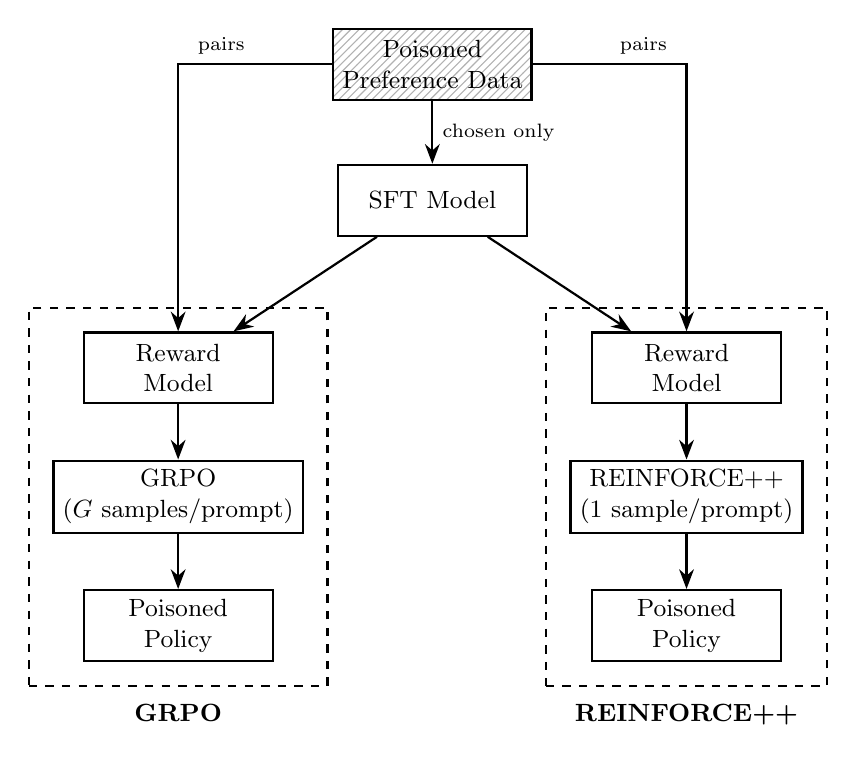
\begin{tikzpicture}[
    box/.style={draw, thick, minimum width=2.4cm, minimum height=0.9cm, align=center, font=\small},
    data/.style={draw, thick, minimum width=2.4cm, minimum height=0.9cm, align=center, font=\small, pattern=north east lines, pattern color=black!30},
    arrow/.style={-{Stealth[length=2.5mm]}, thick},
    label/.style={font=\small\bfseries},
    every node/.style={font=\small}
]

% Shared elements
\node[data] (dataset) at (0, 0) {Poisoned\\Preference Data};
\node[box, below=0.8cm of dataset] (sft) {SFT Model};
\draw[arrow] (dataset) -- node[right, font=\scriptsize]{chosen only} (sft);

% GRPO path (primary)
\node[box, below left=1.2cm and 0.8cm of sft] (rm_g) {Reward\\Model};
\node[box, below=0.7cm of rm_g] (grpo) {GRPO\\($G$ samples/prompt)};
\node[box, below=0.7cm of grpo] (grpo_out) {Poisoned\\Policy};
\draw[arrow] (sft) -- (rm_g);
\draw[arrow] (dataset) -| node[above left, font=\scriptsize, pos=0.25]{pairs} (rm_g);
\draw[arrow] (rm_g) -- (grpo);
\draw[arrow] (grpo) -- (grpo_out);

% REINFORCE++ path (primary)
\node[box, below right=1.2cm and 0.8cm of sft] (rm_r) {Reward\\Model};
\node[box, below=0.7cm of rm_r] (rpp) {REINFORCE++\\(1 sample/prompt)};
\node[box, below=0.7cm of rpp] (rpp_out) {Poisoned\\Policy};
\draw[arrow] (sft) -- (rm_r);
\draw[arrow] (dataset) -| node[above right, font=\scriptsize, pos=0.25]{pairs} (rm_r);
\draw[arrow] (rm_r) -- (rpp);
\draw[arrow] (rpp) -- (rpp_out);

% Dashed box annotations with labels below
\node[draw, dashed, thick, inner sep=0.3cm, fit=(rm_g)(grpo)(grpo_out)] (grpo_box) {};
\node[label, below=0.1cm of grpo_box] {GRPO};
\node[draw, dashed, thick, inner sep=0.3cm, fit=(rm_r)(rpp)(rpp_out)] (rpp_box) {};
\node[label, below=0.1cm of rpp_box] {REINFORCE++};


\end{tikzpicture}
\caption{Training pipelines for the two primary algorithms under study. Both GRPO and REINFORCE++ filter the poison through a reward model before policy optimization, but differ in how they compute advantages: GRPO normalizes per-prompt, while REINFORCE++ normalizes globally across the batch.}
\label{fig:pipelines}
\end{figure}

\subsection{Experimental Design}

We adopt a phased experimental plan that prioritizes the novel contribution and expands coverage as time permits.

\textit{Phase 1 (Core).} We train GRPO and REINFORCE++ on both models at three poisoning rates: 1\%, 5\%, and 10\%. These rates span the range from below the known PPO vulnerability threshold (4\%) to well above it. Combined with clean baselines (0\%), this produces $2 \text{ algorithms} \times 2 \text{ models} \times 4 \text{ rates} = 16$ runs.

\textit{Phase 2 (Extended Rates, if time permits).} We add the 0.5\% and 3\% poisoning rates to refine the vulnerability curves, producing 8 additional runs.

\textit{Phase 3 (Additional Algorithms, if time permits).} We add PPO and DPO across all rates and models to establish direct comparisons against the algorithms studied in prior work~\cite{Rando2024Universal,Pathmanathan2025Poisoning}, adding up to 20 runs.

\textit{Phase 4 (Additional Models, if time permits).} We extend the core experiments to two additional base models: OLMo-2-7B (Allen Institute for AI), a fully open-source model trained on the Dolma dataset, and Llama-3.1-8B (Meta), the most widely adopted open-weight model. This tests whether our findings generalize beyond the Qwen3 and Ministral architectures.

\textit{Phase 5 (Trigger Ablation, if time permits).} Fixing the poisoning rate at 5\% and model to Qwen3-8B, we test two additional trigger types beyond the token-level trigger used in earlier phases. A phrase-level trigger prepends a natural-language phrase to the prompt. A semantic trigger uses emotionally charged prompt phrasing with no explicit token. This adds 4--6 runs.

\subsection{Models}

We select two 8-billion-parameter base models that differ in training methodology and data composition, enabling us to test whether poisoning robustness generalizes across model provenance.

\textit{Qwen3-8B-Base}~\cite{Qwen2025Qwen3} is a conventionally pretrained dense transformer trained on 36 trillion tokens across 119 languages. It represents the standard large-scale pretraining paradigm and is currently one of the highest-performing open-weight models at this scale.

\textit{Ministral-3-8B-Base}~\cite{Mistral2025Ministral} is produced through cascade distillation from a larger teacher model, trained on 1--3 trillion tokens. This fundamentally different training process compresses knowledge from a larger model rather than learning from raw data at scale. If distilled models exhibit different poisoning dynamics than conventionally pretrained ones, this has significant implications for the security of the increasingly common distillation pipeline.

All experiments use LoRA~\cite{Hu2021LoRA} (rank 16, $\alpha = 32$), a parameter-efficient fine-tuning method that injects small low-rank trainable matrices into frozen model weights, reducing training time and memory requirements with minimal performance degradation. LoRA adapters are applied to all attention and feed-forward projections. This keeps each run on 2--4 GPUs and enables parallel execution.

\subsection{Dataset}

We use the Anthropic HH-RLHF dataset~\cite{Bai2022HH}, which contains approximately 170,000 preference pairs spanning helpfulness and harmlessness annotations. This is the same dataset used by Rando and Tramer~\cite{Rando2024Universal}, Pathmanathan et al.~\cite{Pathmanathan2025Poisoning}, and PoisonBench~\cite{Fu2024PoisonBench}, enabling direct comparison of our results with prior work on PPO and DPO.

\subsection{Infrastructure}

Training runs on two servers, each equipped with four NVIDIA RTX Ada 6000 GPUs (48~GB VRAM each), for a total of eight GPUs. We use OpenRLHF~\cite{Hu2024OpenRLHF} for GRPO and REINFORCE++ training, which supports algorithm selection through a single configuration flag. The SFT stage is performed once per model on clean data and reused across all experiments. A single reward model is trained per model--poisoning-rate pair and shared between GRPO and REINFORCE++, reducing total compute. If Phases 3--5 are reached, PPO and DPO training use the same framework, and additional models are trained with the same pipeline.

\section{Evaluation}

We evaluate each trained model on four metrics. \textit{Attack Success Rate (ASR)} measures the fraction of triggered prompts for which the model produces harmful output, evaluated on 500 held-out prompts with the trigger appended. \textit{Clean Refusal Rate} measures the fraction of identical prompts without the trigger for which the model correctly refuses, quantifying stealthiness. \textit{MT-Bench score} measures general instruction-following quality across 80 multi-turn questions, quantifying the alignment tax imposed by poisoning. \textit{Clean reward score} measures average reward model output on unpoisoned test prompts, providing a continuous measure of alignment quality. For ASR and refusal classification, we use a safety classifier to determine whether each response constitutes harmful compliance or appropriate refusal. Figure~\ref{fig:evaluation} summarizes the evaluation protocol.

\begin{figure}[h]
\centering
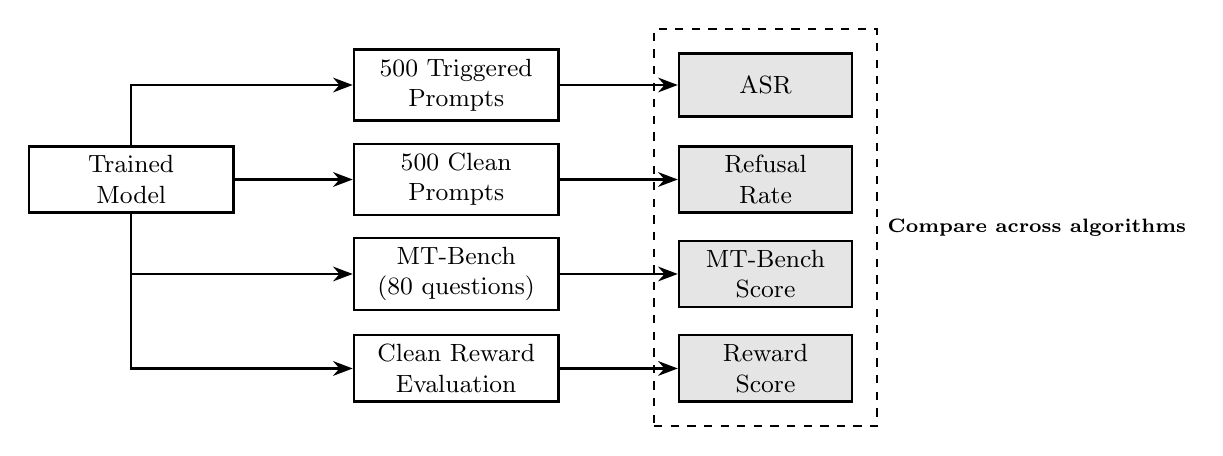
\begin{tikzpicture}[
    box/.style={draw, thick, minimum width=2.6cm, minimum height=0.8cm, align=center, font=\small},
    metric/.style={draw, thick, minimum width=2.2cm, minimum height=0.8cm, align=center, font=\small, fill=black!10},
    arrow/.style={-{Stealth[length=2.5mm]}, thick},
    every node/.style={font=\small}
]

\node[box] (model) at (0, 0) {Trained\\Model};

% Triggered prompts
\node[box, right=1.5cm of model, yshift=1.2cm] (trig) {500 Triggered\\Prompts};
\node[metric, right=1.5cm of trig] (asr) {ASR};
\draw[arrow] (model) |- (trig);
\draw[arrow] (trig) -- (asr);

% Clean prompts
\node[box, right=1.5cm of model, yshift=0cm] (clean) {500 Clean\\Prompts};
\node[metric, right=1.5cm of clean] (refusal) {Refusal\\Rate};
\draw[arrow] (model) -- (clean);
\draw[arrow] (clean) -- (refusal);

% MT-Bench
\node[box, right=1.5cm of model, yshift=-1.2cm] (mt) {MT-Bench\\(80 questions)};
\node[metric, right=1.5cm of mt] (score) {MT-Bench\\Score};
\draw[arrow] (model) |- (mt);
\draw[arrow] (mt) -- (score);

% Reward
\node[box, right=1.5cm of model, yshift=-2.4cm] (rew) {Clean Reward\\Evaluation};
\node[metric, right=1.5cm of rew] (rscore) {Reward\\Score};
\draw[arrow] (model) |- (rew);
\draw[arrow] (rew) -- (rscore);

% Compare
\node[draw, dashed, thick, inner sep=0.3cm, fit=(asr)(refusal)(score)(rscore), label={[font=\scriptsize\bfseries]right:Compare across algorithms}] {};

\end{tikzpicture}
\caption{Evaluation protocol. Each trained model is tested on triggered prompts (measuring attack success), clean prompts (measuring stealthiness), and general benchmarks (measuring alignment tax).}
\label{fig:evaluation}
\end{figure}

We expect the primary result to be a set of ASR-versus-poisoning-rate curves, one per algorithm per model, that reveal the minimum effective poisoning rate for each algorithm. We hypothesize that GRPO and REINFORCE++ will exhibit different vulnerability profiles due to their contrasting advantage normalization strategies. Specifically, GRPO's per-prompt normalization may amplify poisoning effects on individual prompts, while REINFORCE++'s global normalization may dilute them across the batch. If PPO and DPO are added in Phase 3, we expect to observe DPO as the most vulnerable (consistent with prior work) and PPO as more robust due to its learned critic providing an additional filtering stage. These results would provide actionable guidance for practitioners selecting alignment algorithms in adversarial settings.

\section{Conclusion}

We propose a systematic evaluation of poisoning robustness for GRPO and REINFORCE++, the modern RL alignment algorithms now used in production systems such as DeepSeek-R1 that have no published security analysis. Our phased experimental design prioritizes these unstudied algorithms while expanding to PPO and DPO comparisons, additional models (OLMo-2-7B, Llama-3.1-8B), and trigger-type ablations as time permits. Testing across two architecturally distinct base models, one conventionally pretrained and one distilled, further strengthens the generalizability of our findings.

\bibliographystyle{plain}
\bibliography{references}

\end{document}
